%!TEX root = ../main.tex

\documentclass[../main.tex]{subfiles}
\begin{document}

\chapter{Single Robot Coverage}
\label{chapter:single_robot_coverage}

This chapter addresses the problem of the single agent coverage. In this section, we motivate the problem, state the problem, and propose a solution.

First, we state the problem of coverage in its most general form.
\begin{problem}[Minimum Cost Coverage Path Planning]
\label{problem:min_cost_cpp}
	Given a workspace $W$, a robot with dynamics, and a coverage footprint mapping $\mathcal{M}(q)$, compute a path $p^*\in P$ such that
	\begin{equation}
	\label{condition:full_coverage}
	\begin{aligned}
		& \bigcup_{q\in p^*}\mathcal{M}(q)=\mathcal{C},\\
		& \mathcal{E}(p^*)\leq\mathcal{E}(p), \forall p\in P.
	\end{aligned}
	\end{equation}
\end{problem}

In Problem~\ref{problem:min_cost_cpp}, a workspace $W$, a robot with dynamics, and a coverage footprint are given. The objective is to compute a path that lies entirely in the free configuration space of the robot such that the footprint of the path is equal to the coverable space of the environment and the cost of the path is minimized.

A number of aspects of this problem makes it difficult. For instance, the set of feasible paths $P$ contain infinitely many paths. Also, it is difficult to directly check the satisfiability of conditions~(\ref{condition:full_coverage}). In this work, we rely on heuristics by making justified restrictions to the feasible set to simplify the problem.


\section{Problem Statement}
\label{sec:single_problem_statement}

From our experience working with robotic companies and from some of the literature, we have observed that one of the most efficient paths for many types of robots are paths that are completely straight line segments. Here, efficiency could be interpreted in various ways. For instance, a battery powered differential drive robot traveling in a straight line has to do work to execute a turn. This is because it needs to slow down or speed up some of its wheels. Once it finishes executing a turn, it needs to speed up again by using energy from the battery. Hence, any turns on its path leads to decrease in energy efficiency, which is undesirable. Other examples include area scanning via a fixed wing UAV. Whenever a UAV has to make a turn while executing a coverage path, its scanning equipment, which is typically points downwards and fixed to the airframe, will swivel and point in a different direction~\cite{frew2004vision}. This reduces the quality of the coverage and will usually result in a second pass. Hence, turns in the scanning applications reduce the efficiency of coverage paths.

Motivated by these observations, we aim to compute coverage paths with minimum turning. There is a related problem of the minimum bend TSP~\cite{wagner2001approximation}. However, we aim to avoid the issue of discretization that is associated with the TSP approaches as outlined in the previous section.

To that end, we restrict the set of feasible paths to the set of feasible but segmented paths as shown in Figure~\ref{fig:nonsegmented_vs_segmented}. The set of feasible segmented path is defined in Definition~\ref{definition:segmented_feasible_paths}.
\begin{definition}[Set of Feasible Segmented Path]
\label{definition:segmented_feasible_paths}
A set of feasible segmented paths is defined as:
	\begin{equation}
	\begin{aligned}
		P_{\text{segmented}}=\{p_i\ |\ p_i\subseteq Q_{\text{free}},\  p_i=\{s_1,t_1,s_2,t_2,\dots,s_n,t_n\}\}\subseteq P.
	\end{aligned}
	\end{equation}
\end{definition}
where $s_i$ refers to straight line segments and $t_i$ refers to the transition segments.

\begin{figure}
	\centering
	\begin{subfigure}{0.5\linewidth}
		\centering
		\subfile{img/chapter_3/non_segmented_path}
	\end{subfigure}%
	\begin{subfigure}{0.5\linewidth}
		\centering
		\subfile{img/chapter_3/segmented_path}
	\end{subfigure}
	\caption{An example of non-segmented path and a segmented path.}
	\label{fig:nonsegmented_vs_segmented}
\end{figure}

Problem~\ref{problem:min_cost_cpp} is modified accordingly to specify the search space of feasible paths.
\begin{problem}[Minimum Cost Coverage Path Planning with Straight Line Segments]
\label{problem:min_cost_cpp_with_lines}
	Given a workspace $W$, a robot with dynamics, and a coverage footprint mapping $\mathcal{M}(q)$, compute a path $p^*\in P_{\text{segmented}}$ such that
	\begin{equation}
	\label{condition:full_coverage_2}
	\begin{aligned}
		& \bigcup_{q\in p^*}\mathcal{M}(q)=\mathcal{C},\\
		& \mathcal{E}(p^*)\leq\mathcal{E}(p), \forall p\in P.
	\end{aligned}
	\end{equation}
\end{problem}

[Connect Segmented Coverage Path Planning Problem to Minimum Number of Lines Problem]

Our earlier assumption relies on the fact that straight line segments are the cheapest paths for a robot. In other words, any transition segments connecting point $a$ and $b$ are going to have higher cost than a straight line segment connecting points $a$ and $b$. As such, it is intuitive to try to minimize the number of transition segments in the path. Note the structure of paths in $P_{\text{segmented}}$, i.e., $p_i=\{s_1,t_1,s_2,t_2,\dots,s_n,t_n\}$. Minimizing the number of straight line segment in the path is equivalent to minimizing the number of transition segments.

In literature, Problem~\ref{problem:min_cost_cpp_with_lines} is a lot more common. Moreover, a very common approach is to utilize a type of path called Boustrophedon paths~\cite{choset2000coverage}. With this approach, the whole workspace or a number of subregions of the workspace are covered via straight line segments placed parallel to each other. It should be noted that by itself, the Boustrophedon path does not achieve complete coverage even for convex polygons. A wall following part is required to achieve full coverage. However, since the wall following component is a fixed cost part of the path, it is useful from the analysis standpoint to look at just Boustrophedon component of the path.

For demonstrative purposes, we will state a simpler problem where a simple solution exists in literature. Suppose we have the following problem:
\begin{problem}[Minimum Cost Coverage Path Planning with Parallel Straight Line Segments]
\label{problem:min_cost_cpp_with_parllel_lines}
	Given a workspace $W$ and a robot with dynamics, compute a path $p^*\in P_{\text{segmented}}$ such that $\{s_1,s_2,\dots,s_n\}$ is a set of parallel straight line segments $|S|$ is minimized.
\end{problem} 

One of the solutions to this problem is presented in the work by Huang~\cite{Huang2001optimal} and the solution involves choosing the orientation for the set of parallel straight line segments that minimizes the \emph{altitude}. Since we will use this notion of altitude extensively, we will formally define it here.

\textbf{Minimum Altitude:} For convex polygons, the altitude in direction $\theta$ is defined as the minimum distance between two parallel lines angled at $\theta+\frac{\pi}{2}$ with respect to the $x$-axis such that all vertices of the convex polygon are contained between these two lines \cite{Huang2001optimal}. The altitude of the polygon in Figure~\ref{fig:transition_point} is the distance between lines $e_i$ and $h_i$. This notion can be extended to general polygons. The method of obtaining $\theta$ altitude for a general polygon is shown in Algorithm~\ref{alg:altitude}. Figure \ref{fig:altitude} provides an example of this procedure. In the example, the altitude is $x_1 + 2x_2 + 3x_3 + 2x_4 + x_5$. Note that if $r$ is the radius of the footprint of the robot and $\alpha$ is the altitude of a polygon along $\theta$ then the total number of lines required for complete coverage in direction $\theta$ is
\begin{equation}
	n=\floor*{\frac{\alpha}{2r}}.
\end{equation}

\begin{figure}
	\centering
	\begin{subfigure}{0.5\linewidth}
		\centering
		\subfile{img/chapter_3/reorient_solution_1}
	\end{subfigure}%
	\begin{subfigure}{0.5\linewidth}
		\centering
		\subfile{img/chapter_3/reorient_solution_2}
	\end{subfigure}
	\caption{Polygon regions where lines can be reoriented.}
	\label{fig:reorder_regions}
\end{figure}

\begin{algorithm}
	\caption{$\operatorname{get\_general\_altitude}(P, \theta)$}
	\label{alg:altitude}
	\begin{algorithmic}[1]
		\REQUIRE Polygon $P=\{Z_0, Z_1,\ldots\}$, direction $\theta$.
			\STATE $\operatorname{counter}\gets 0$, $\alpha\gets 0$
			\STATE Rotate $P$ by $-\theta$ to align direction with $x$-axis.
			\STATE Sort all vertices in $P$ by their  $x$-coordinates
			\FOR{each $v_i$ in the sorted list}
				\STATE $\alpha\gets \alpha+\operatorname{counter}\times(x_{v_{i}}-x_{v_{i-1}})$ 
				\IF{both vertices adjacent to $v_i$ are on right}
					\STATE Increment $\operatorname{counter}$ by 1
				\ELSIF{both vertices adjacent to $v_i$ are on left}
					\STATE Decrement $\operatorname{counter}$ by 1
				\ENDIF
			\ENDFOR
			\RETURN $\alpha$
		%\ENDPROCEDURE 
	\end{algorithmic}
\end{algorithm}

However, as demonstrated in Figure~\ref{fig:reorder_regions}, this solution is clearly not optimal. There are certain regions in the polygon where a subset of straight line segments could be reoriented resulting in a smaller set. In other words, the minimum altitude of the overall workspace can be reduced by considering the sum of minimum altitudes of a certain partition of a polygon. As such, we propose the following problem.

\begin{problem}[Minimum Altitude Decomposition]
\label{problem:min_lin_num_decomp}
Given a polygonal workspace $W$, find $k$ and $w_1,w_2,\ldots,w_k$ such that $\sum^k_{i=1}\alpha^*(w_i)$ is minimized where $\bigcup^k_{i=1}w_i=P$.
\end{problem}

Of course, once Problem~\ref{problem:min_lin_num_decomp} is solved, we have a set of straight line segments. We still need to generate a path. Hence, we introduce a second problem.

\begin{problem}[Minimum Cost Tour]
\label{problem:min_tour}
Given a polygon $P$ and a set of lines $\Gamma$, generate a matrix $M$ of transition costs between any pair of elements of $\Gamma$. Find a tour of $\Gamma$ such that cost of the tour is minimized.
\end{problem}

The following sections will introduce our approach to these problems.

\section{Min Altitude Polygon Decomposition for Coverage Planning}
\label{sec:decomposition}

This section covers our solution to Problem~\ref{prob:min_lin_num_decomp_3}. Section~\ref{sec:preliminaries} introduces decomposition related terminology that is needed to present our decomposition method.

\subsubsection{Min Altitude Decomposition}
This section outlines the approach to Problem~\ref{prob:min_lin_num_decomp_3}. The overall steps of the process are described in Algorithm~\ref{alg:min_alt_decomposition}.
\begin{algorithm}
	\caption{$\operatorname{min\_alt\_decomposition}(P)$}
	\label{alg:min_alt_decomposition}
	\begin{algorithmic}[1]
		\REQUIRE Polygon $P=\{Z_0,Z_1,\ldots\}$
			\STATE $D\gets$ any convex decomposition of $P$	\label{line:cvx_decomp}
			\REPEAT
				\STATE Re-optimize a cut from $D$ \label{line:opt_cut_2}
				\STATE Update cost of the decomposition \label{line:update_cost}
			\UNTIL{stopping criteria is met}
	\end{algorithmic}
\end{algorithm}

\begin{figure}
	\centering
	\subfile{img/chapter_3/altitude}
	\caption{Process of measuring altitude with $\theta$ equal to 0.}
	\label{fig:altitude}
\end{figure}


Algorithm~\ref{alg:min_alt_decomposition} accepts a polygon as the input. On Line~\ref{line:cvx_decomp}, initial decomposition is generated using any convex decomposition technique. The rest of the algorithm attempts to re-optimize this decomposition in order to decrease the overall altitude. Re-optimization steps on Lines~\ref{line:opt_cut_2} and \ref{line:update_cost} are performed until the cost of the decomposition no longer decreases. The core of Algorithm~\ref{alg:min_alt_decomposition} is the procedure for making optimal decomposing cuts shown in Line~\ref{line:opt_cut_2}. The procedure for making optimal decomposing cuts is introduced in Section~\ref{sec:alt_cut_decomposition}.

\subsection{Optimal Decomposing Cut}
\label{sec:alt_cut_decomposition}
The re-optimization step operates on a polygon with a reflex vertex. This polygon is formed by removing the previous cut that was made by a convex decomposition. Our algorithm will either generate a new cut or no cut depending on what is optimal with respect to the altitude of the polygon. We do this by searching for optimal decomposing cuts. The algorithm for doing that is shown in Algorithm~\ref{alg:optimal_cut}. The procedure operates on a single chain and a specified reflex vertex in that chain. On Line~\ref{line:cut_cut_space}, a cut space is generated for the reflex vertex, which provides a set of potential cuts. Two polygons, $P_{\ell}$ and $P_r$ are formed by initializing the cut at the first point of the cut space on Line~\ref{line:cut_two_polygons}. Two sets of altitude directions are generated on Lines~\ref{line:cut_two_sets}-\ref{line:cut_two_sets_2} based on the two polygons. On Lines~\ref{line:opt_cut_for}-\ref{line:opt_cut_end_for}, candidates for a cut are found for each combination of directions and each straight segment of the cut space. Before moving on to the next straight segment of the cut space, $P_l$ is modified to include $S_i$ in its boundary. $P_r$ is modified to exclude $S_i$ from its boundary. The checked straight segment may also add a new altitude direction which has to be accounted for. These operations are carried out on Lines~\ref{line:cut_modify_1}-\ref{line:opt_cut_end_for}. The algorithm returns the cut that has the lowest cost.

\begin{algorithm}
	\caption{$\operatorname{find\_optimal\_cut}(P, v)$}
	\label{alg:optimal_cut}
	\begin{algorithmic}[1]
		\REQUIRE Polygon $P=\{Z_0\}$, reflex vertex $v$
			\STATE $A_{\ell}\gets\emptyset,\;A_r\gets\emptyset$, $U\gets\emptyset$
			\STATE Find cut space $S$ for $v$	\label{line:cut_cut_space}
			\STATE $P_{\ell},P_r\gets$ polygons after cut at first endpoint of $S$ \label{line:cut_two_polygons}
			\STATE $\Theta_{\ell}\gets$set of directions $\theta$ orthogonal to edges of $P_{\ell}$ \label{line:cut_two_sets}
			\STATE $\Theta_r\gets$set of directions $\theta$ orthogonal to edges of $P_r$ \label{line:cut_two_sets_2}
			\FOR{each $S_i\in S$} \label{line:opt_cut_for}
				\FOR{each $\operatorname{dir}_{\ell}\in \Theta_{\ell}$}
					\FOR{each $\operatorname{dir}_r\in \Theta_r$}
						\STATE $u\gets\operatorname{get\_cands}(P_{\ell}$, $P_r$, $S_i$, $\operatorname{dir}_{\ell}$, $\operatorname{dir}_r)$ \label{line:get_cands}
						\STATE Add tuple $(u, \operatorname{dir}_{\ell}, \operatorname{dir}_r)$ to $U$
					\ENDFOR
				\ENDFOR
				\STATE Modify $P_{\ell}$ by adding $S_i$ to its boundary \label{line:cut_modify_1}
				\STATE Modify $P_r$ by removing $S_i$ from its boundary
				\STATE Modify $\Theta_{\ell},\Theta_r$ if new $\theta$ was introduced by $S_i$ \label{line:opt_cut_end_for}
			\ENDFOR 
			\STATE Compute costs for all tuples $(u, \operatorname{dir}_{\ell}, \operatorname{dir}_r)\in U$
			\RETURN Lowest cost element from $U$
		%\ENDPROCEDURE 
	\end{algorithmic}
\end{algorithm}
The important step in Algorithm~\ref{alg:optimal_cut} is the function $\operatorname{get\_cands}$ on Line~\ref{line:get_cands}. This function finds candidates for a cut. The procedure is described in Algorithm \ref{alg:find_candidate}.
Lines~\ref{line:cand_trans_pt}-\ref{line:cand_trans_pt_2} of Algorithm~\ref{alg:find_candidate} obtain special points on $S_i$ called transition points for each polygon and altitude direction. These points are associated with the point on $S_i$ that minimize the sum of altitudes. Transition points are formally introduced in Section~\ref{sec:proof_of_correctness}. On Line~\ref{line:cand_if}, both transition points result in equal value, so one of them is returned. Otherwise, a transition point is chosen based on the direction which has the most significant increase in altitude. This is determined by the altitude direction and the orientation of the cut space segment.
\begin{algorithm}
	\caption{$\operatorname{get\_cands}(P_{\ell}, P_r, S_i, \operatorname{dir}_{\ell}, \operatorname{dir}_r)$}
	\label{alg:find_candidate}
	\begin{algorithmic}[1]
		\REQUIRE Two polygons, edge on cut space, two directions
			\STATE $t_1\gets$ transition point on $S_i$ w.r.t $\operatorname{dir}_{\ell}$	\label{line:cand_trans_pt}
			\STATE $t_2\gets$ transition point on $S_i$ w.r.t $\operatorname{dir}_r$ \label{line:cand_trans_pt_2}
			\IF{$t_1$ is further along cut space then $t_2$}\label{line:cand_if}
				\STATE $U\gets(t_1, \operatorname{dir}_{\ell}, \operatorname{dir}_r)$
			\ELSE \label{line:cand_else}
				\STATE $\delta\alpha_{\ell}\gets |\operatorname{proj}_{\operatorname{dir}_{\ell}}S_i|$
				\STATE $\delta\alpha_r\gets |\operatorname{proj}_{\operatorname{dir}_r}S_i|$

				\IF{$\delta\alpha_{\ell}>\delta\alpha_r$}
					\STATE $U\gets(t_1, \operatorname{dir}_{\ell}, \operatorname{dir}_r)$
				\ELSE
					\STATE $U\gets(t_2, \operatorname{dir}_{\ell}, \operatorname{dir}_r)$
				\ENDIF
			\ENDIF
	\end{algorithmic}
\end{algorithm}

\subsection{Proof of Correctness}
\label{sec:proof_of_correctness}

Algorithm~\ref{alg:optimal_cut} provides an optimal decomposing cut. This section proves optimality of this claim.

\begin{claim}
Given a polygon $P$ and a reflex vertex $v$, Algorithm~\ref{alg:optimal_cut} returns a decomposing cut forming two new polygons that minimize $\alpha^*(P_{\ell})+\alpha^*(P_r)$.
\end{claim}

The rest of this section will provide proof for this claim. Suppose a polygon $P$ is given with a reflex vertex $v$. By Definition~\ref{def:decomposing_cut}, a decomposing cut generates two new polygons, $P_{\ell}$ and $P_r$. The sets of all edges of $P_{\ell}$ and $P_r$ are $E_{\ell}$ and $E_r$ respectively. We are interested in studying how a choice of a cut affects the altitudes of $P_{\ell}$ and $P_r$. Let us parameterize the orientation of a cut with respect to $t$. There is a function $f:\mathbb{R}\to\mathbb{R}^2$ which maps a parameter $t\in[0,1]$ to a point $x\in\mathbb{R}^2$ on the cut space. Let $w_1$ be a point on cut space when $t=0$ corresponding to a cut on edge $e_1$. See Figure~%\ref{fig:cut}. Define $\alpha_i(t)$ as a function that measures altitude orthogonal to edge $e_i$.

Define the two sets of altitudes as follows:
\begin{equation}
\begin{aligned}
\label{eq:set_of_altitudes}
&A_{\ell}=\{\alpha_{\ell,i}(t)\ |\ i\in\{1,\ldots,|E_{\ell}|\},\\
&A_{r}=\{\alpha_{r,i}(t)\ |\ i\in\{1,\ldots,|E_r|\}.
\end{aligned}
\end{equation}


Note, each element $\alpha_{\ell,i}(t)\in A_{\ell}$ and $\alpha_{r,i}(t)\in A_r$ is a semi-continuous function of $t$, with discontinuities occurring only when the cut sweeps past a pinch vertex in the cut space as shown in Figure~\ref{fig:pinch_vertex}.

\begin{figure}
	\centering
	\subfile{img/chapter_3/pinch_vertex}
	\caption{An example of a pinch vertex at $v_p$.}
	\label{fig:pinch_vertex}
\end{figure}

\begin{lemma}
There exists a $t\in[0,1]$ that minimizes $\alpha_{\ell,i}(t)+\alpha_{r,j}(t)$.
\end{lemma}
\begin{proof}
For $P_{\ell}$ and $P_r$, the minimum altitudes are
\begin{equation}
\begin{aligned}
\alpha_{1,\min}(t)=\min(\alpha_{1,1}(t),\ldots,\alpha_{1,n}(t)),\\
\alpha_{2,\min}(t)=\min(\alpha_{2,1}(t),\ldots,\alpha_{2,m}(t)).
\end{aligned}
\end{equation}


These functions are semi-continuous. Furthermore, the objective of the optimization is the sum of two minimum altitudes of the two polygons,
\begin{equation}
\begin{aligned}
\label{eq:sum_min}
\alpha_{1,\min}(t)+\alpha_{2,\min}(t).
\end{aligned}
\end{equation}

The quantity in Equation~\ref{eq:sum_min} is also semi-continuous. Furthermore, since $t\in[0,1]$ is in a compact set, the minimum of Equation \ref{eq:sum_min} exists by the extension of the extreme value theorem.
\end{proof}

Fix $S_i\in S$ and let $f(a)$ and $f(b)$ correspond to end points of $S_i$ as shown in Figure~\ref{fig:transition_point}. Consider $\alpha_{1,i}(t)\in A_{\ell}$ which is measured with respect to $e_i$. Construct a line $h_{i}$ that is parallel to $e_i$ that passes through $v$. Denote $f(t_{1,\operatorname{trans}})$ as the point on $S_i$ that intersects $h_i$. Let us refer to this point as a transition point. There are three possibilities:
\begin{enumerate}
	\item $t_{1,\operatorname{trans}}\geq b$,
	\item $t_{1,\operatorname{trans}}\leq a$,
	\item $t_{1,\operatorname{trans}}\in(a,b)$.
\end{enumerate} 
These cases are shown in Figure~\ref{fig:altitude_cases_pl}. In the first case, $\alpha_{1,i}(t)$ remains constant for all $t\in[a,b]$. In the second case, $\alpha_{1,i}(t)$ is an increasing linear function for all $t\in[a,b]$. In the third case, $\alpha_{1,i}(t)$ remains constant for all $t\in[a,t_{1,\operatorname{trans}}]$ and becomes an increasing linear function for all $t\in[t_{1,\operatorname{trans}},b]$.

%\begin{definition}[Transition points]
%Define $t_{\operatorname{trans}}$ to be the transition points of $\alpha_{1,i}(t)$. In other words, transition point is $t$ after which $\alpha_{1,i}(t)$ start increasing.
%\end{definition}

\begin{figure}
	\centering
	\subfile{img/chapter_3/transition_point}
	\caption{An example of a transition point.}
	\label{fig:transition_point}
\end{figure}


Now, we perform similar analysis for the same $S_i$ but for the right polygon $P_r$. The results are almost identical where the only difference is the behavior of $\alpha_{2,i}(t)$ in three cases outlined above. Figure~\ref{fig:altitude_cases_pr} demonstrates these cases. In the first case, $\alpha_{2,i}(t)$ is a decreasing linear function for all $t\in[a,b]$. In the second case, $\alpha_{2,i}(t)$ remains constant for all $t\in[a,b]$. In the third case, $\alpha_{2,i}(t)$ is a decreasing linear function for all $t\in[a,t_{2,\operatorname{trans}}]$ and remains constant for all $t\in[t_{2,\operatorname{trans}},b]$. Hence, for each $S_i$ and a combination of altitudes, $\alpha_{1,i}(t)$ and $\alpha_{2,j}(t)$, we have two transition points, $\{t_{1,\operatorname{trans}}, t_{2,\operatorname{trans}}\}$.
\begin{lemma}
\label{lemma:min_at_trans_pts}
For a given $S_i$, altitudes $\alpha_{1,i}(t)$ and $\alpha_{2,j}(t)$, a minimizer of $\alpha_{1,i}(t)+\alpha_{2,j}(t)$ is $t\in\{t_{1,\operatorname{trans}}, t_{2,\operatorname{trans}}\}$.
\end{lemma}
\begin{proof}
Observe that $\alpha_{1,i}(t)+\alpha_{2,j}(t)$ is a sum of piece-wise linear functions.  For any combination of two cases depicted in Figure~\ref{fig:altitude_cases_pl} and Figure~\ref{fig:altitude_cases_pr}, there are two cases to consider when looking for the minimizer of the sum.

If $t_{1,\operatorname{trans}}\geq t_{2,\operatorname{trans}}$ then the optimal happens at $t_{2,\operatorname{trans}}$. If $t_{1,\operatorname{trans}}<t_{2,\operatorname{trans}}$ then the optimal depends on the slopes of the linear functions. Let $\delta\alpha_{\ell}$ and $\delta\alpha_r$ be the slopes of the left and right altitudes respectively. If $\delta\alpha_{\ell}>\delta\alpha_r$ then the optimum point is at $t_{1,\operatorname{trans}}$. Otherwise, it is at $t_{2,\operatorname{trans}}$.

There is an altitude associated with the cut itself in $A_{\ell}$ and in $A_r$ that does not exhibit the same properties that were discussed previously. However, by the properties shown by Huang\cite{Huang2001optimal}, this altitude varies as a piece-wise continuous sinusoidal function of $\phi$ where $\phi$ is the angle of a cut with respect to $e_1$. This means the altitude for $P_{\ell}$ is minimized when either the cut is parallel to one of the edges of $P_{\ell}$ or when $t\in\{a,b\}$. Likewise for $P_r$. However, when the cut is parallel to one of the edges of $P_{\ell}$ or $P_r$, this means that the altitude is identical to another altitude in the set $A_{\ell}$ or $A_r$. Since these altitudes are checked first, we only have to check both transition points at $f(a)$ and $f(b)$.
\end{proof}

By Lemma \ref{lemma:min_at_trans_pts}, it is enough to compute the cost of each transition point for each $S_i\in S$ and all combinations of elements from $A_{\ell}$ and $A_r$ and pick one point with lowest cost. This is the procedure described in Algorithm~\ref{alg:optimal_cut}.

\section{Computational Complexity}
Algorithm~\ref{alg:find_candidate} is $\mathbb{O}(1)$. Algorithm~\ref{alg:optimal_cut} is more complicated. The inner most loop is $\mathbb{O}(n)$ where $n$ is the number of edges in a polygon. So is the second inner most loop. Hence, the run time of two inner loops is $\mathbb{O}(n^2)$ where $n$ is the number of edges in the polygon. The first for loop runs in $\mathbb{O}(n)$ where $n$ is the number of edges in a polygon. Hence, the overall polygon runs in $\mathbb{O}(n^3)$ where $n$ is the number of edges in a polygon.

\begin{figure}
	\centering
	\begin{subfigure}{0.45\linewidth}
		\centering
		\subfile{img/chapter_3/altitude_func_pl_1}
		\caption{\label{fig:altitude_case_i}}
	\end{subfigure}%
	\quad
	\begin{subfigure}{0.45\linewidth}
		\centering
		\subfile{img/chapter_3/altitude_func_pl_2}
		\caption{\label{fig:altitude_case_ii}}
	\end{subfigure}
	\begin{subfigure}{0.45\linewidth}
		\centering
		\subfile{img/chapter_3/altitude_func_pl_2}
		\caption{\label{fig:altitude_case_iii}}
	\end{subfigure}
	\caption{Three cases of altitude behavior for $P_{\ell}$.}
	\label{fig:altitude_cases_pl}
\end{figure}

\begin{figure}
	\centering
	\begin{subfigure}{0.45\linewidth}
		\centering
		\subfile{img/chapter_3/altitude_func_pr_1}
		\caption{\label{fig:altitude_case_pr_i}}
	\end{subfigure}%
	\quad
	\begin{subfigure}{0.45\linewidth}
		\centering
		\subfile{img/chapter_3/altitude_func_pr_2}
		\caption{\label{fig:altitude_case_pr_ii}}
	\end{subfigure}
	\begin{subfigure}{0.45\linewidth}
		\centering
		\subfile{img/chapter_3/altitude_func_pr_3}
		\caption{\label{fig:altitude_case_pr_iii}}
	\end{subfigure}
	\caption{Three cases of altitude behavior for $P_r$.}
	\label{fig:altitude_cases_pr}
\end{figure}


\section{Improvements to Decomposition}
\label{sec:improvment}
The most computational intensive task in Algorithm~\ref{alg:optimal_cut}  is computing cut candidates for each pair of altitude directions (Line~\ref{line:opt_cut_for}-\ref{line:opt_cut_end_for}). The computation load can be reduced by only evaluating a subset of direction pairs as follows.

Define $\underline{P}_{\ell}$ and $\underline{P}_{r}$ to be the polygons on either side of the cone of bisection. It is important to note that the cone of bisection is not a part of these polygons. We compute look-up tables of altitudes for every direction for $\underline{P}_{\ell}$ and $\underline{P}_{r}$ separately such that $\alpha(\underline{P}_{\ell},\text{dir}_1)$ returns the altitude of $\underline{P}_{\ell}$ in direction $\text{dir}_1$. These look-up tables represent the best case scenario for a pair of directions. In the main loop of Algorithm~\ref{alg:optimal_cut}, we keep track of the best altitude so far. A check is added to the main loop such that for a pair of directions, $\text{dir}_1$ and $\text{dir}_2$, if $\alpha(\underline{P}_{\ell},\operatorname{dir}_1)+\alpha(\underline{P}_{r},\operatorname{dir}_2)$ is larger than the best altitude so far, then this pair of directions cannot be optimal, and no further computation is needed.

\subsection{GTSP Tour Generation}
\label{sec:gtsp_tour}

Given a polygon $P$, Algorithm~\ref{alg:min_alt_decomposition} is called on $P$, resulting in a set $D$ of polygons. For each $P_i\in D$, we generate the minimum set $\Gamma_i$ of straight segment footprints. Note, each $\gamma_j\in\Gamma_i$ has two possible traversal directions. We refer to the choice of this direction as $\gamma_j^1$ or $\gamma_j^2$  as shown in Figure~\ref{fig:traversal_directions}. Define $\operatorname{cost}(\gamma_i^m, \gamma_j^l)$ as the robot transition cost from region $\gamma_i$ in $m$ direction to region $\gamma_j$ in $l$ direction where $m,l\in\{1,2\}$ and $i,j\in\{1,\ldots,k\},i\neq j$. This transition cost takes the dynamics of the robot into account. Computing this cost for each pair $\gamma_i^m, \gamma_j^l$, a complete graph $G=(V,E,w)$ is constructed where each vertex $v\in V$ represents $\gamma^m_i$ for some $m\in\{1,2\}$ and $i=\{1,\ldots,k\}$, each edge $e=\{v,z\}$ in $E$ represents transition between vertices $v$ and $z$, and weights represent robot transition costs between vertices. Furthermore, $V$ is partitioned into sets $\{\gamma_i^1,\gamma_i^2\}$ for $i=\{1,\ldots,k\}$. The graph $G$ and the partition define the GTSP instance, and a GTSP tour on this graph gives a coverage path for the robot. 

\begin{figure}
	\centering
	\subfile{img/chapter_3/gtsp_i}
	\caption{Two possible traversal directions for line $\gamma_j$.}
	\label{fig:traversal_directions}
\end{figure}
\begin{figure}
	\centering
	\subfile{img/chapter_3/gtsp_ii}
	\caption{Two possible traversal directions for line $\gamma_j$.}
	\label{fig:cost}
\end{figure}

\subsection{Simulations}
\label{sec:simulation}
Our decomposition algorithm was implemented in Python. The algorithm was implemented with the help of computational geometry libraries including Shapely\footnote{The Shapely library is available at \url{https://github.com/Toblerity/Shapely}} and Visilibity%\cite{VisiLibity:08}. The heuristic solver GLKH~\cite{helsgaun2000effective} was used as a GTSP solver. Transition costs between segments were computed assuming a Dubins' vehicle model.

Our method was compared to two other approaches. In the first method we use an approximate point decomposition of the workspace from~\cite{arkin2000approximation}. Each point is assigned eight headings. These headings represent possible traversal directions for that point. Finally, the GTSP tour of minimum cost is computed as in%~\cite{le2012dubins}. In the second method, we compute the coverage path as in Section~\ref{sec:gtsp_tour}, but where the re-optimization procedure is not performed on the initial decomposition. For the initial decomposition, a Python library for greedy convex decomposition is used, based on~\cite{fernandez2008practical}. We tested all approaches on four different workspaces of similar size but various complexity. The workspaces are based on test environments used in~\cite{choi2009online}.

%\begin{table}
%	\centering
%	\begin{tabular}{@{} l rrrr l rrrr l rrrr l@{}}
%		\toprule
%		%\cline{2-7}		
%		& \multicolumn{4}{c}{Point Decomposition} & \phantom{a} & \multicolumn{4}{c}{Greedy Decomposition} & \phantom{a} & \multicolumn{4}{c}{Min Alt Decomposition}\\
%		\cmidrule{2-5} 		\cmidrule{7-10}  \cmidrule{12-15} 
%		& Size & Time & Length & Area & & Size & Time & Length & Area & & Size & Time & Length & Area \\
%		\midrule
%		Shape 1 & 7144 & 2h & 312.6 & 87.8\% & & 96 & \bf{2s} & \bf{231.0} & 91.6\% & & \bf{78} & 2s & 242.3 & \bf{95.1\%}\\
%		%\hline
%		Shape 2 & 7288  & 2h & 306.3 & 86.9\% & & 86 & \bf{2s} & \bf{216.8} & 84.6\% & & \bf{80} & 7s & 228.9 & \bf{91.7\%} \\
		%\hline 
%		Shape 3 & 7464 & 2h & 349.3 & 88.3\% & & 136 & \bf{6s} & \bf{226.9} & 79.8\% & & \bf{92} & 15s & 228.1 & \bf{89.1\%} \\
%		Shape 4 & 6736 & 2h & 312.2 & 85.1\% & & 116 & \bf{3s} & \bf{226.5} & 88.1\% & & \bf{88} & 13s & 234.4 & \bf{93.5\%}\\
%
%		\bottomrule
		%\hline

%	\end{tabular}
%	\caption{Decomposition methods comparison for multiple test shapes.}
%	\label{table:performance}
%\end{table}

\begin{table}
	\centering
	\begin{tabular}{@{} l rrrr l rrrr l rrrr l@{}}
		\toprule
		%\cline{2-7}		
		& \multicolumn{4}{c}{Point Decomposition} & \phantom{a} & \multicolumn{4}{c}{Greedy Decomposition} & \phantom{a} & \multicolumn{4}{c}{Min Alt Decomposition}\\
		\cmidrule{2-5} 		\cmidrule{7-10}  \cmidrule{12-15} 
		& Size & Time & Length & Area & & Size & Time & Length & Area & & Size & Time & Length & Area \\
		\midrule
		Shape 1 & 7144 & 2h & 312.6 & 87.8\% & & 96 & \bf{2s} & \bf{231.0} & 91.6\% & & \bf{78} & 2s & 242.3 & \bf{95.1\%}\\
		%\hline
		Shape 2 & 7288  & 2h & 306.3 & 86.9\% & & 86 & \bf{2s} & \bf{216.8} & 84.6\% & & \bf{80} & 7s & 228.9 & \bf{91.7\%} \\
		%\hline 
		Shape 3 & 7464 & 2h & 349.3 & 88.3\% & & 136 & \bf{6s} & \bf{226.9} & 79.8\% & & \bf{92} & 15s & 228.1 & \bf{89.1\%} \\
		Shape 4 & 6736 & 2h & 312.2 & 85.1\% & & 116 & \bf{3s} & \bf{226.5} & 88.1\% & & \bf{88} & 13s & 234.4 & \bf{93.5\%}\\

		\bottomrule
		%\hline

	\end{tabular}
	\caption{Decomposition methods comparison for multiple test shapes.}
	\label{table:performance}
\end{table}


Performance figures of all three methods are shown in Table~\ref{table:performance}. We compare four characteristics of the three approaches: 1) the size of the GTSP instance, 2) the execution time from start to finish, 3) the total length of the tour, and 4) the area covered by the coverage path as percentage of the total area of the polygon. We note that in all four test shapes, our method reduced the number of turns in the final coverage path. This is shown in the reduction in GTSP size, which is equivalent to the reduction in number of straight line segments. Naturally, since our method uses greedy decomposition as a starting point, it runs more slowly then the pure greedy approach. On average, out method is about three times slower than the greedy approach. However, it is faster then the point decomposition by a factor of 100. 

It is worth noting that the overall path lengths are slightly shorter with the greedy decomposition compared to our method. However, this factor is mostly attributed to the fact that greedy decomposition produces many regions whose area is small relative to the size of the footprint. These regions are typically very narrow, which makes it difficult to place lines inside those regions that cover most of the area. Decompositions that produce excessive number of such regions results in a significant portion of the total area of the polygon uncovered. Our method produces fewer regions and leaves less area uncovered. From Table~\ref{table:performance}, the uncovered area left by our method is on average half of the uncovered area left by the greedy approach. It is worth noting that point decomposition in some cases covers less area than the competing algorithms. However, this occurrence is primarily due to our method for generating the approximate decomposition, which does not place any coverage footprints at a distance of less than $r$ from the boundary, leading to uncovered areas near polygon boundaries.

Figure~\ref{fig:coverage_results} shows the resultant paths for three different approaches. The line segments are orange and green segments show Dubins transition costs. Note that green segments do not necessarily indicate the path of the robot but rather show the cost associated with the transition. The red lines highlight shared edges of adjacent polygons in the decomposition. The first column of figures show the point decomposition. The second column of figures show the greedy decomposition technique. And the last column shows our re-optimization technique. 

From Figure~\ref{fig:coverage_results} we can see that our method significantly reduces the number of polygons compared to the greedy decomposition. Inefficiencies in the GTSP tour occur due to the very large size of the GTSP instance, which poses a challenge for the heuristic GLKH solver.

\begin{figure*}
		\centering
		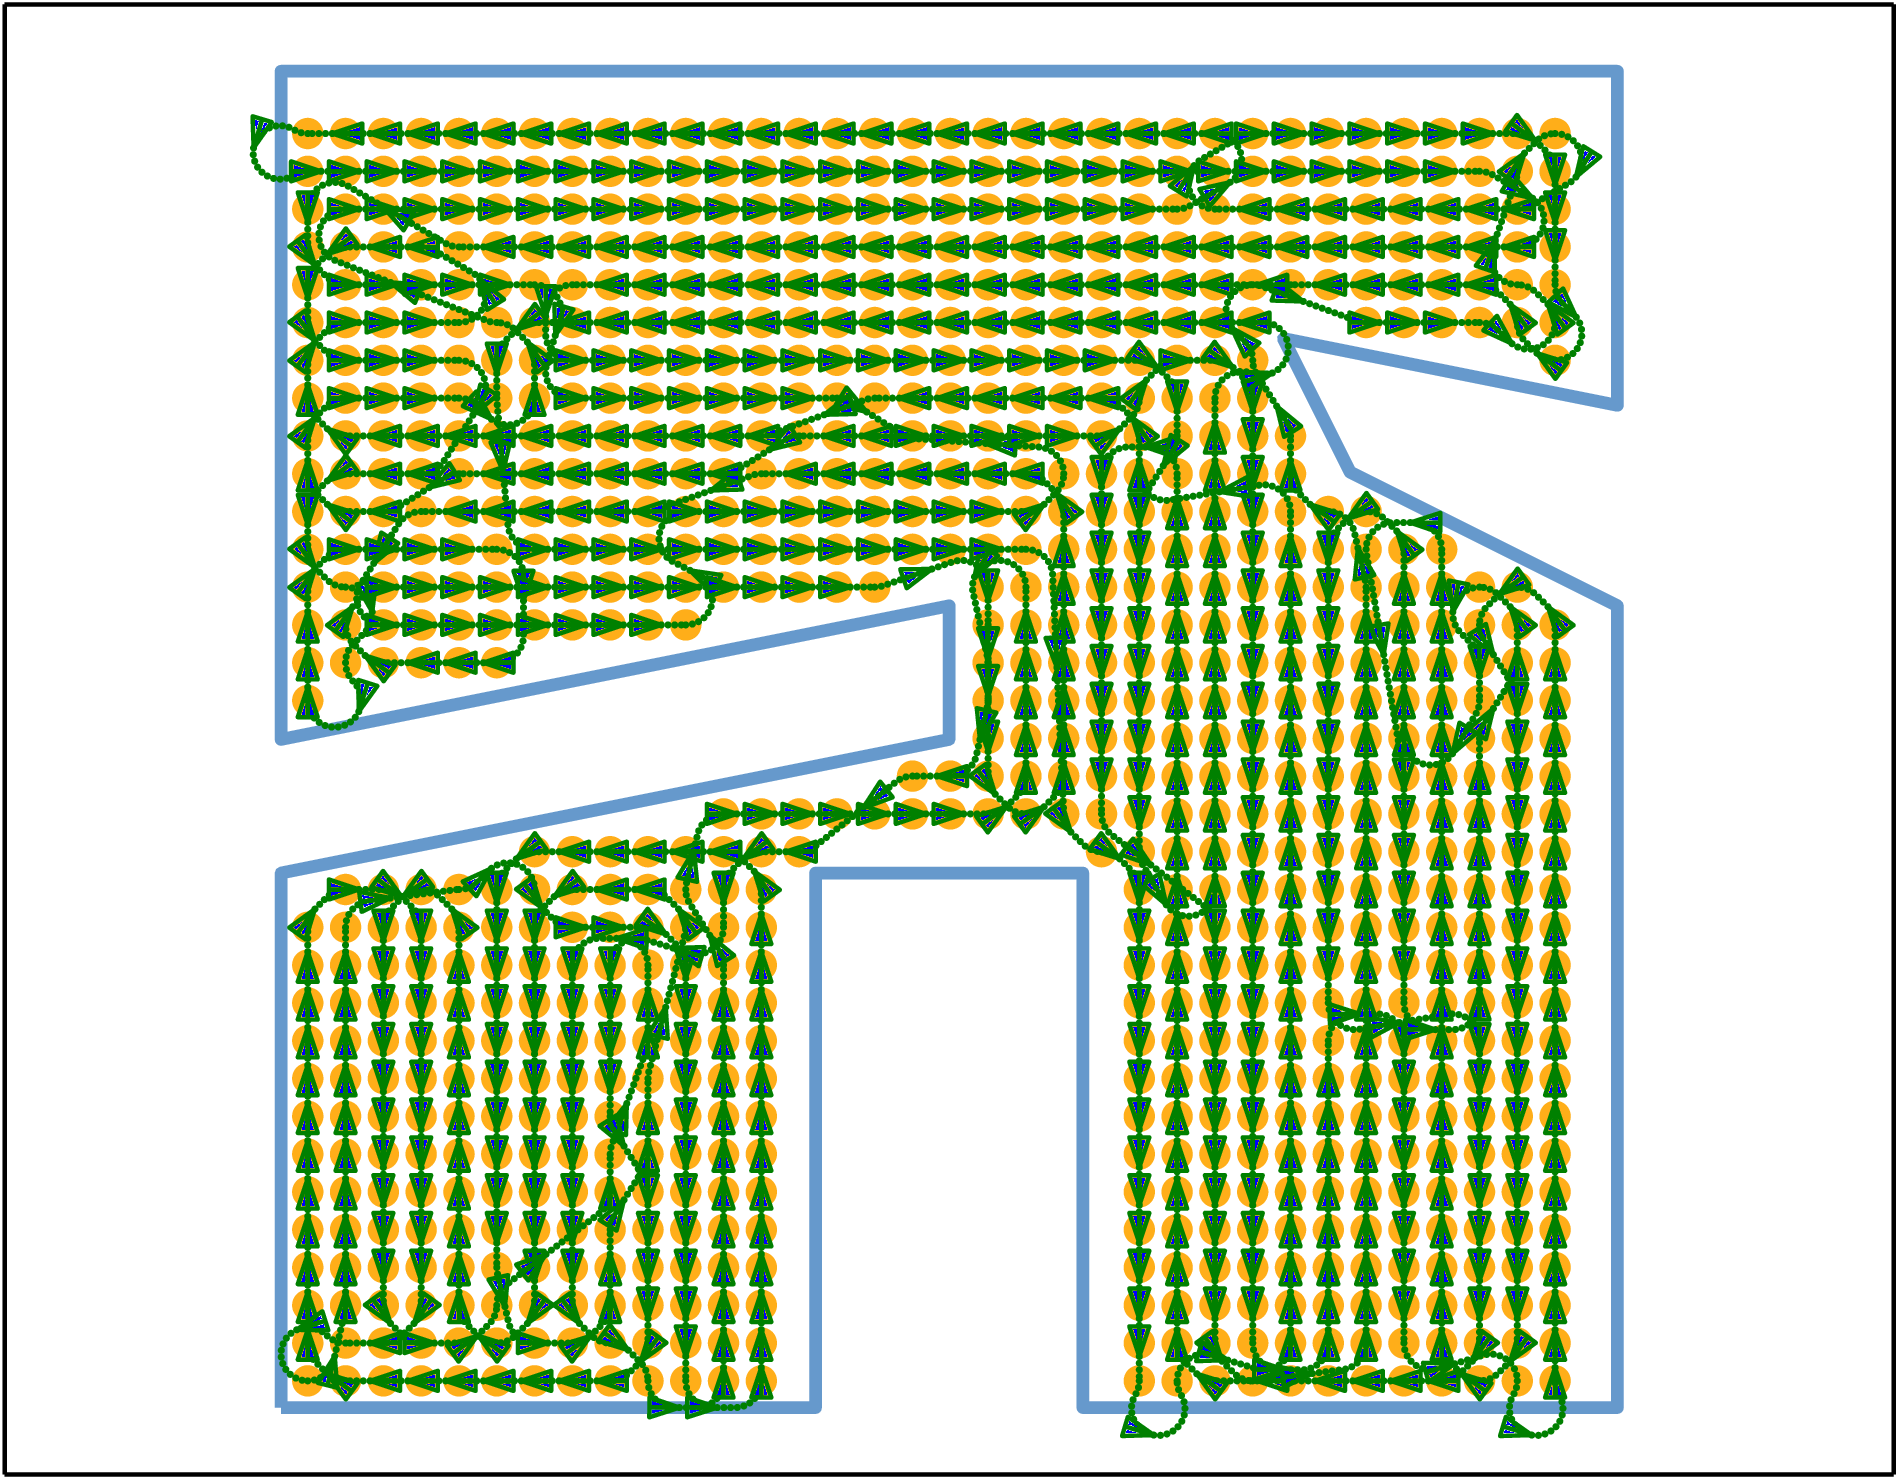
\includegraphics[width=0.3\textwidth]{img/chapter_3/point_10_coverage.png}% 
		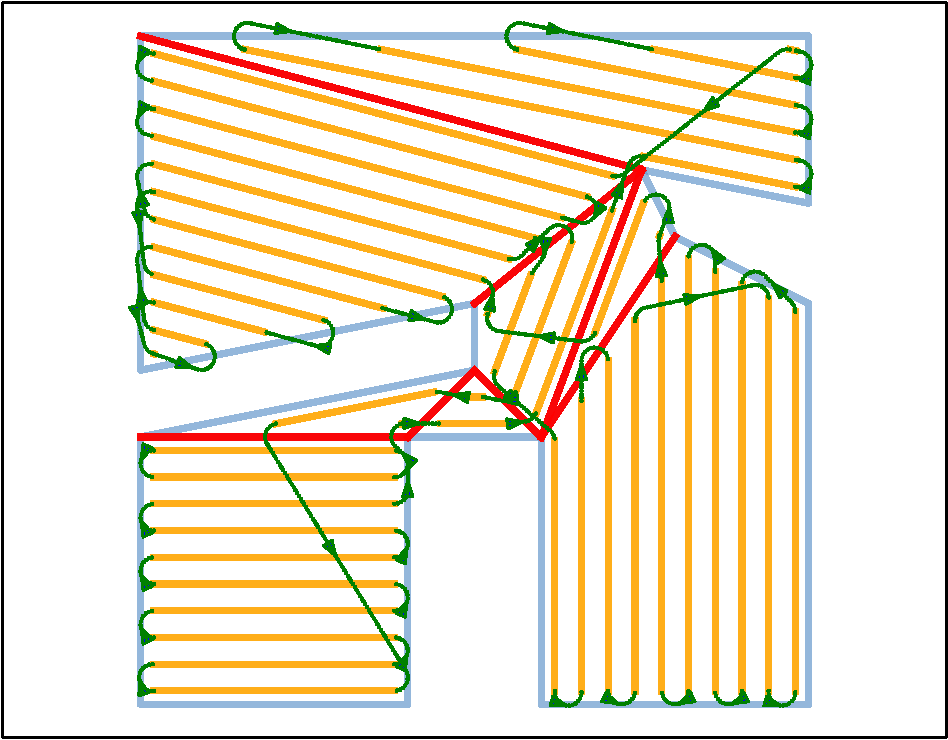
\includegraphics[width=0.3\textwidth]{img/chapter_3/greedy_10_coverage.pdf}% 
		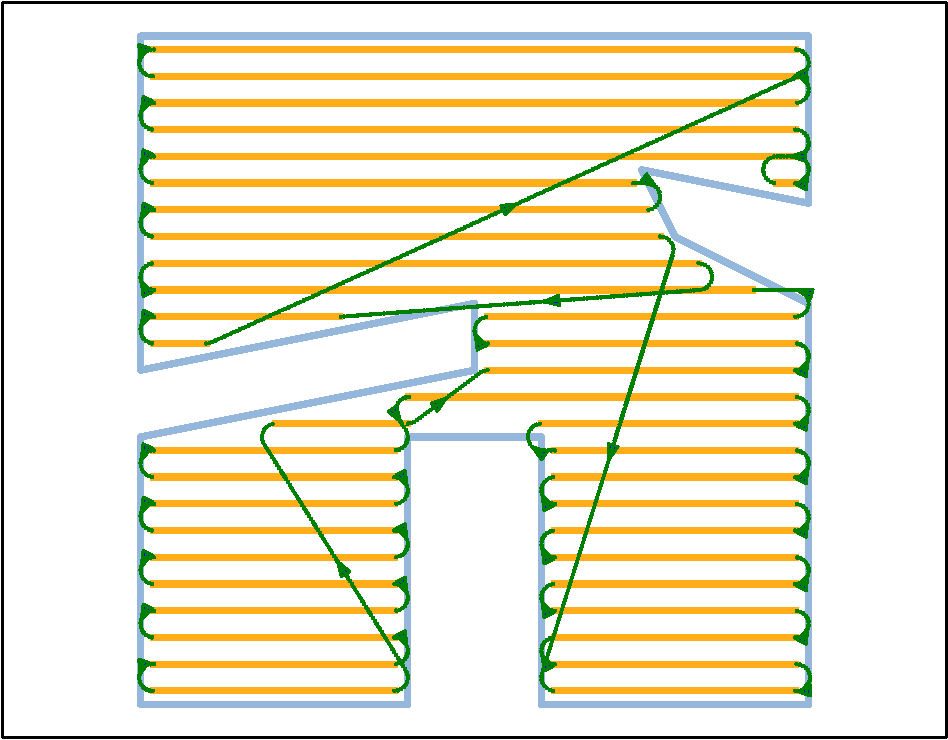
\includegraphics[width=0.3\textwidth]{img/chapter_3/min_10_coverage.pdf}

		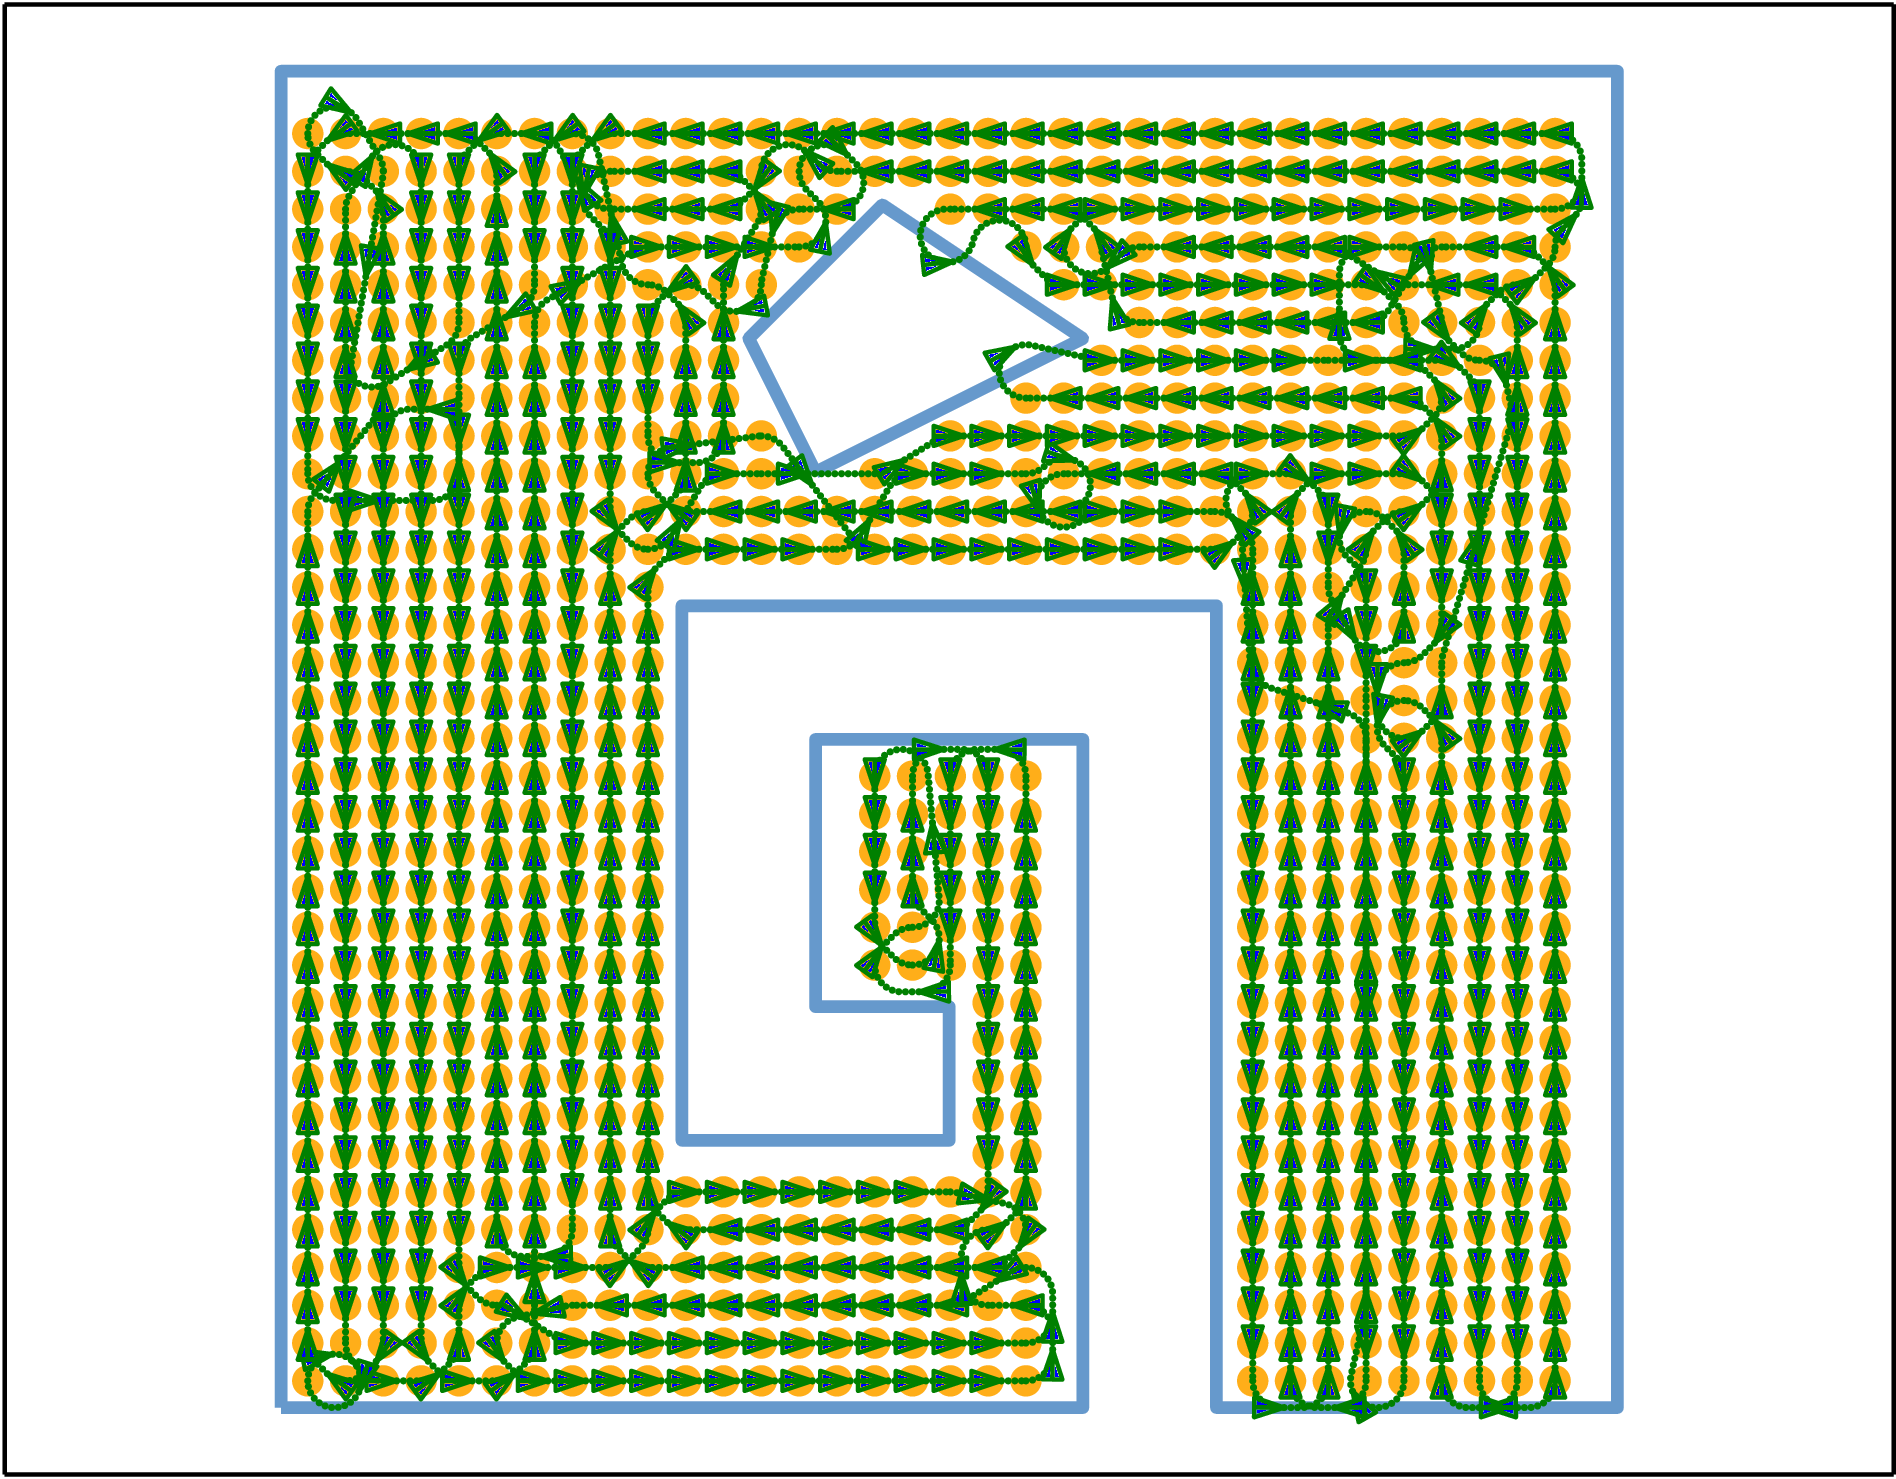
\includegraphics[width=0.3\textwidth]{img/chapter_3/point_11_coverage.png}% 	
		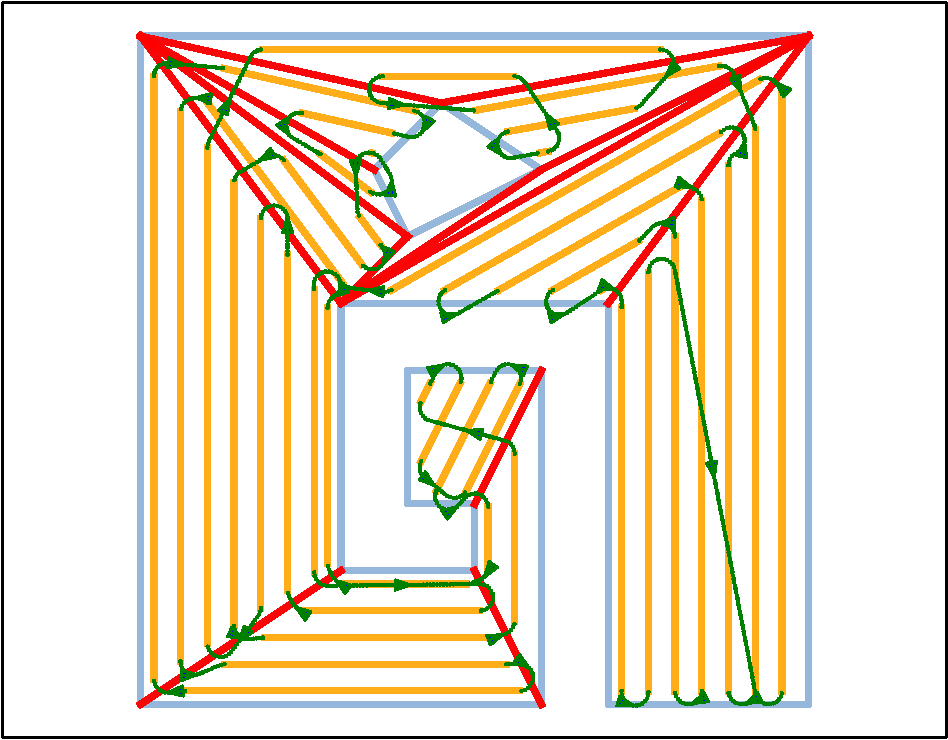
\includegraphics[width=0.3\textwidth]{img/chapter_3/greedy_11_coverage.pdf}%
		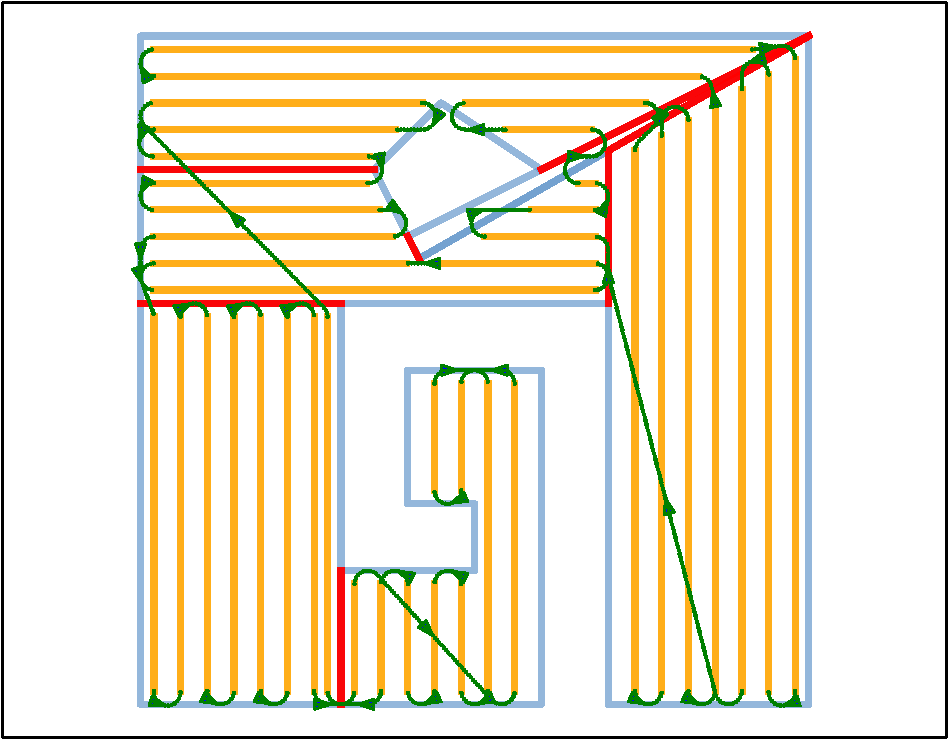
\includegraphics[width=0.3\textwidth]{img/chapter_3/min_11_coverage.pdf}

		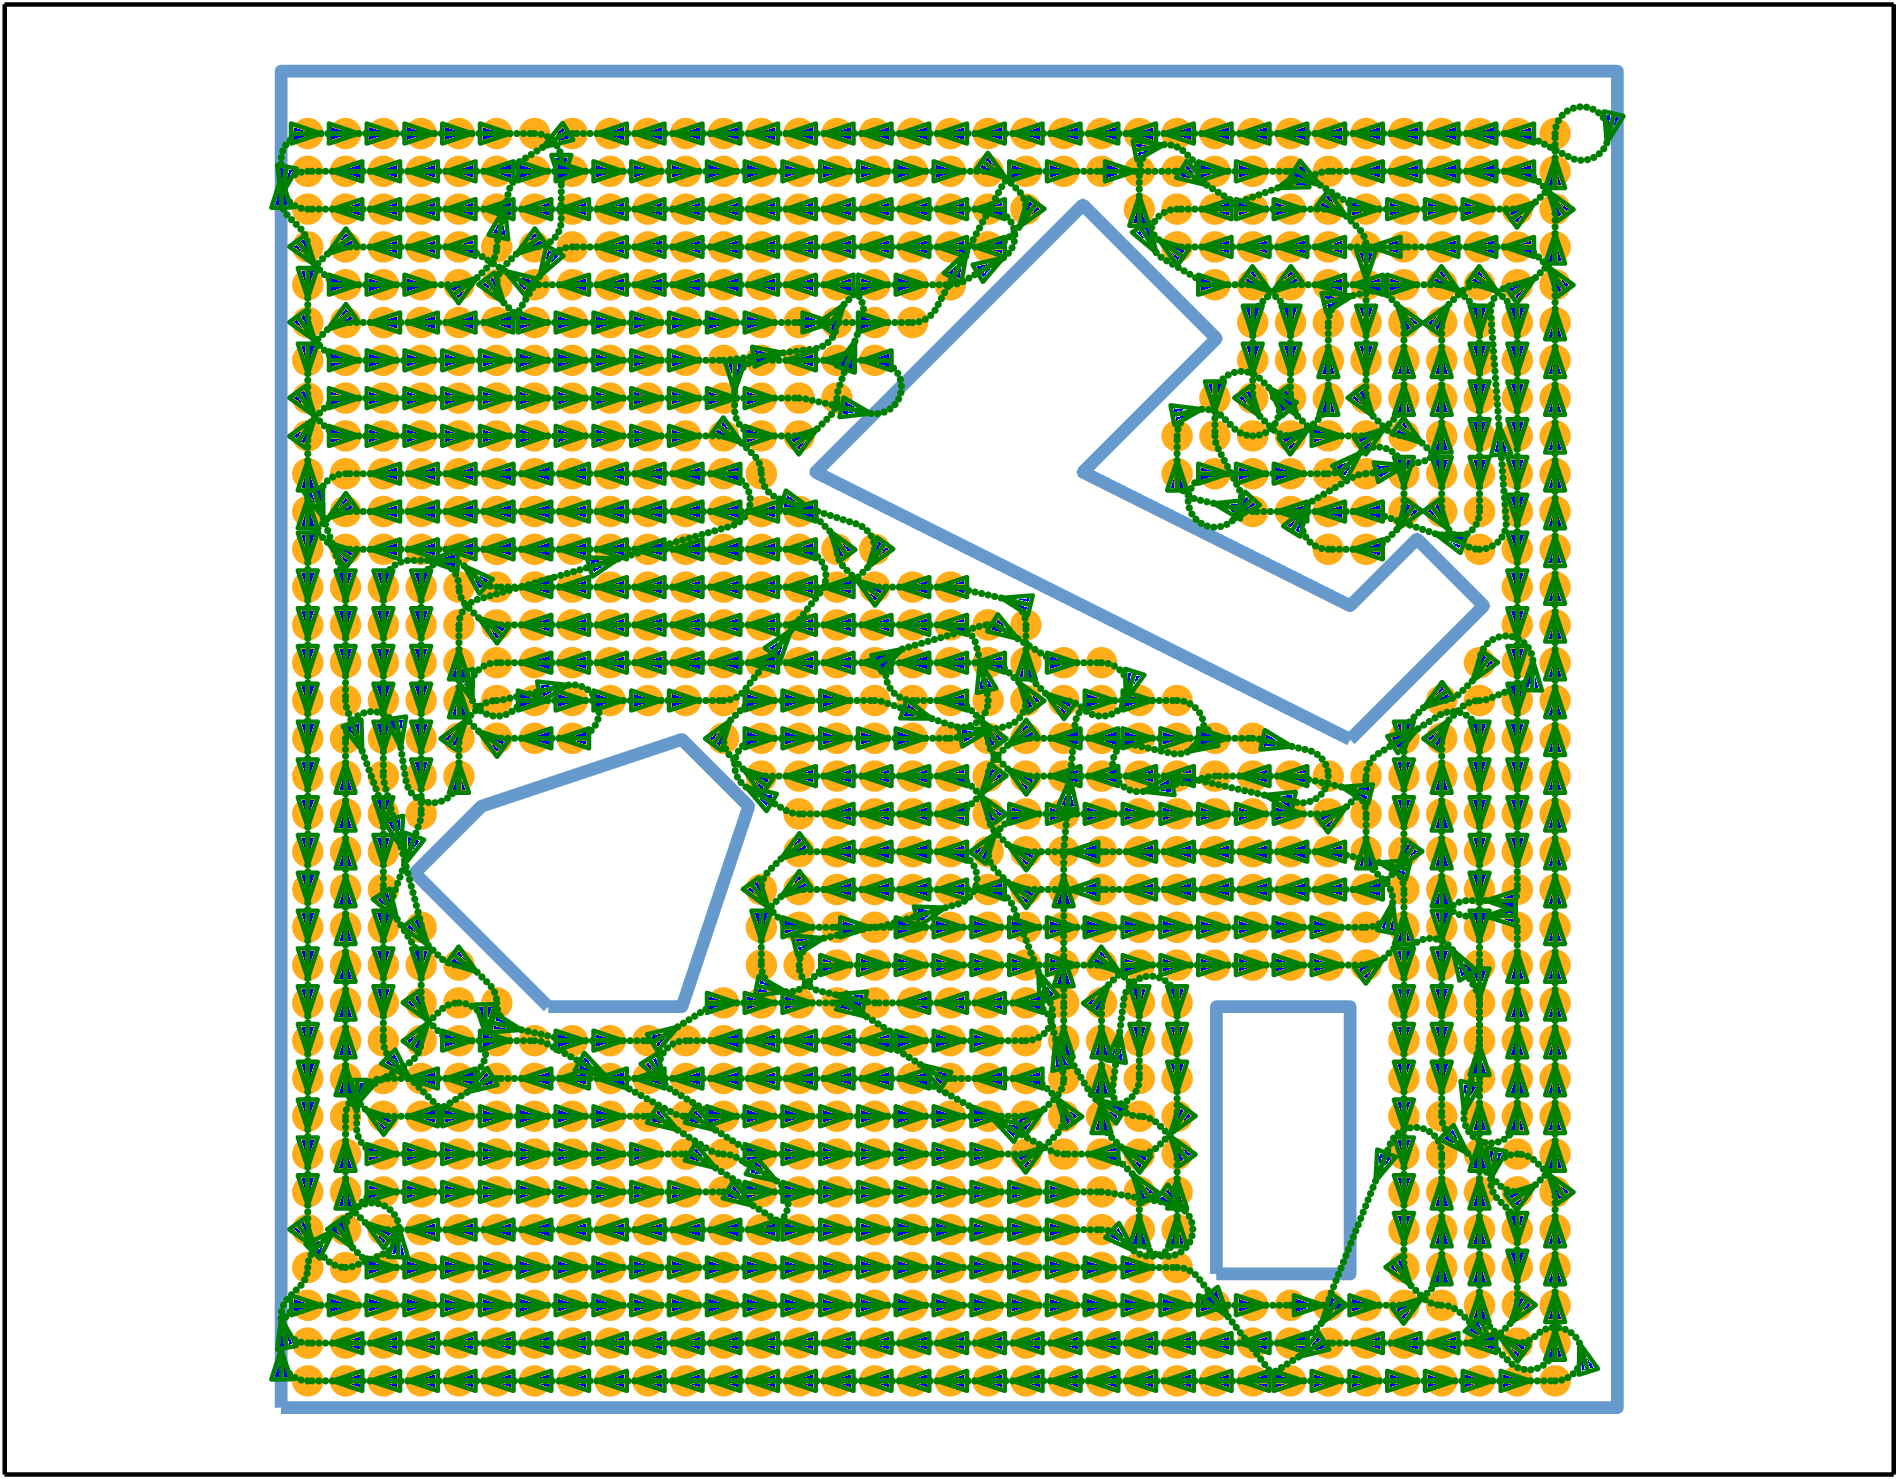
\includegraphics[width=0.3\textwidth]{img/chapter_3/point_12_coverage.png}%
		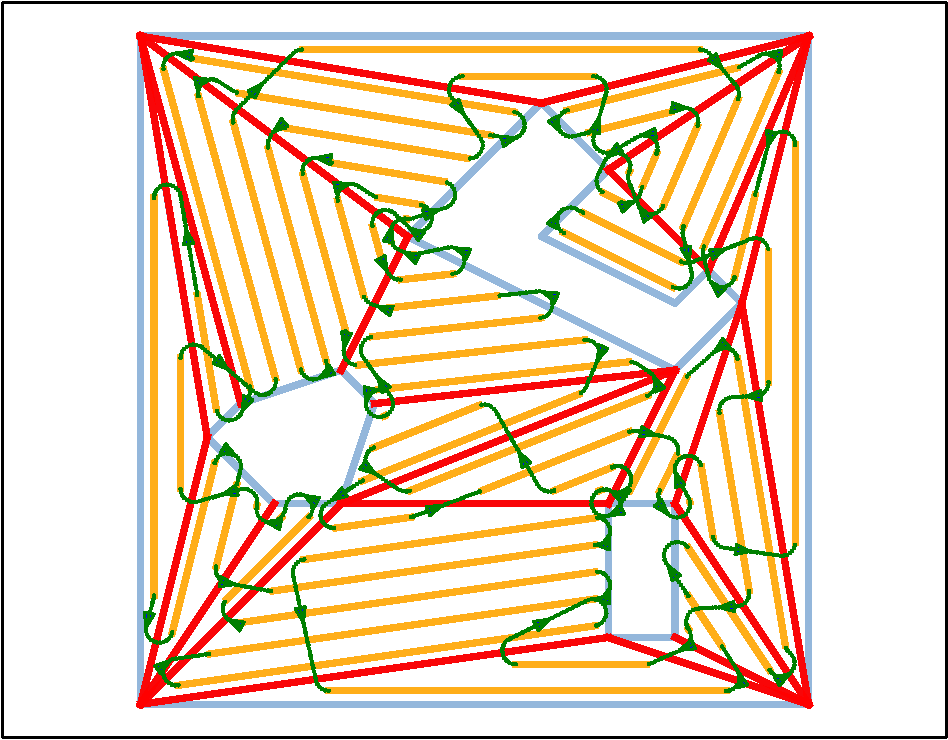
\includegraphics[width=0.3\textwidth]{img/chapter_3/greedy_12_coverage.pdf}%
		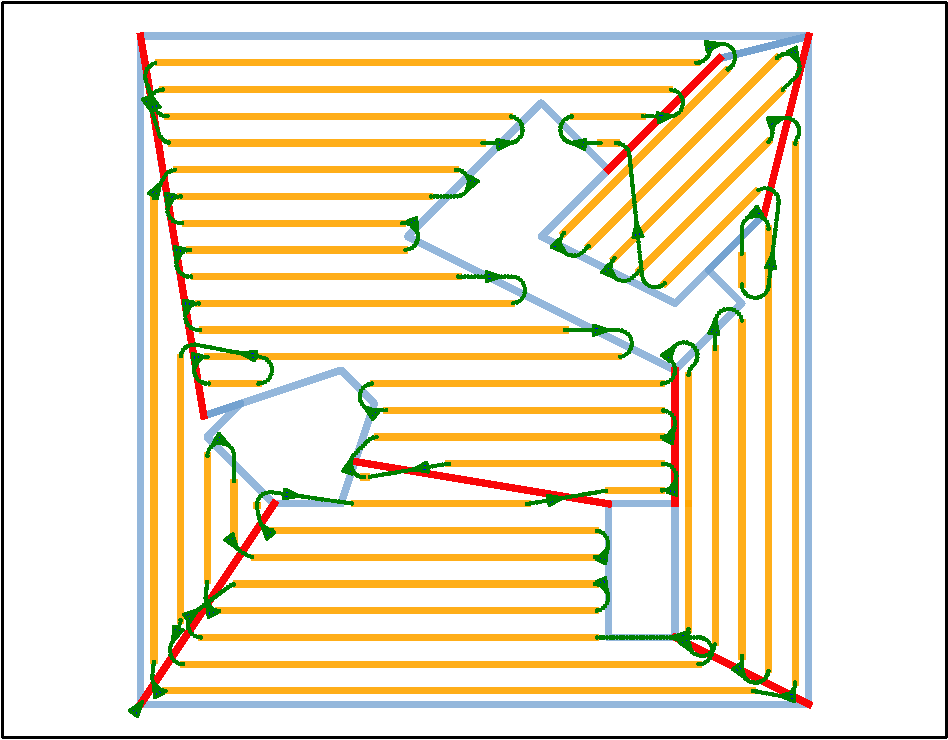
\includegraphics[width=0.3\textwidth]{img/chapter_3/min_12_coverage.pdf}

		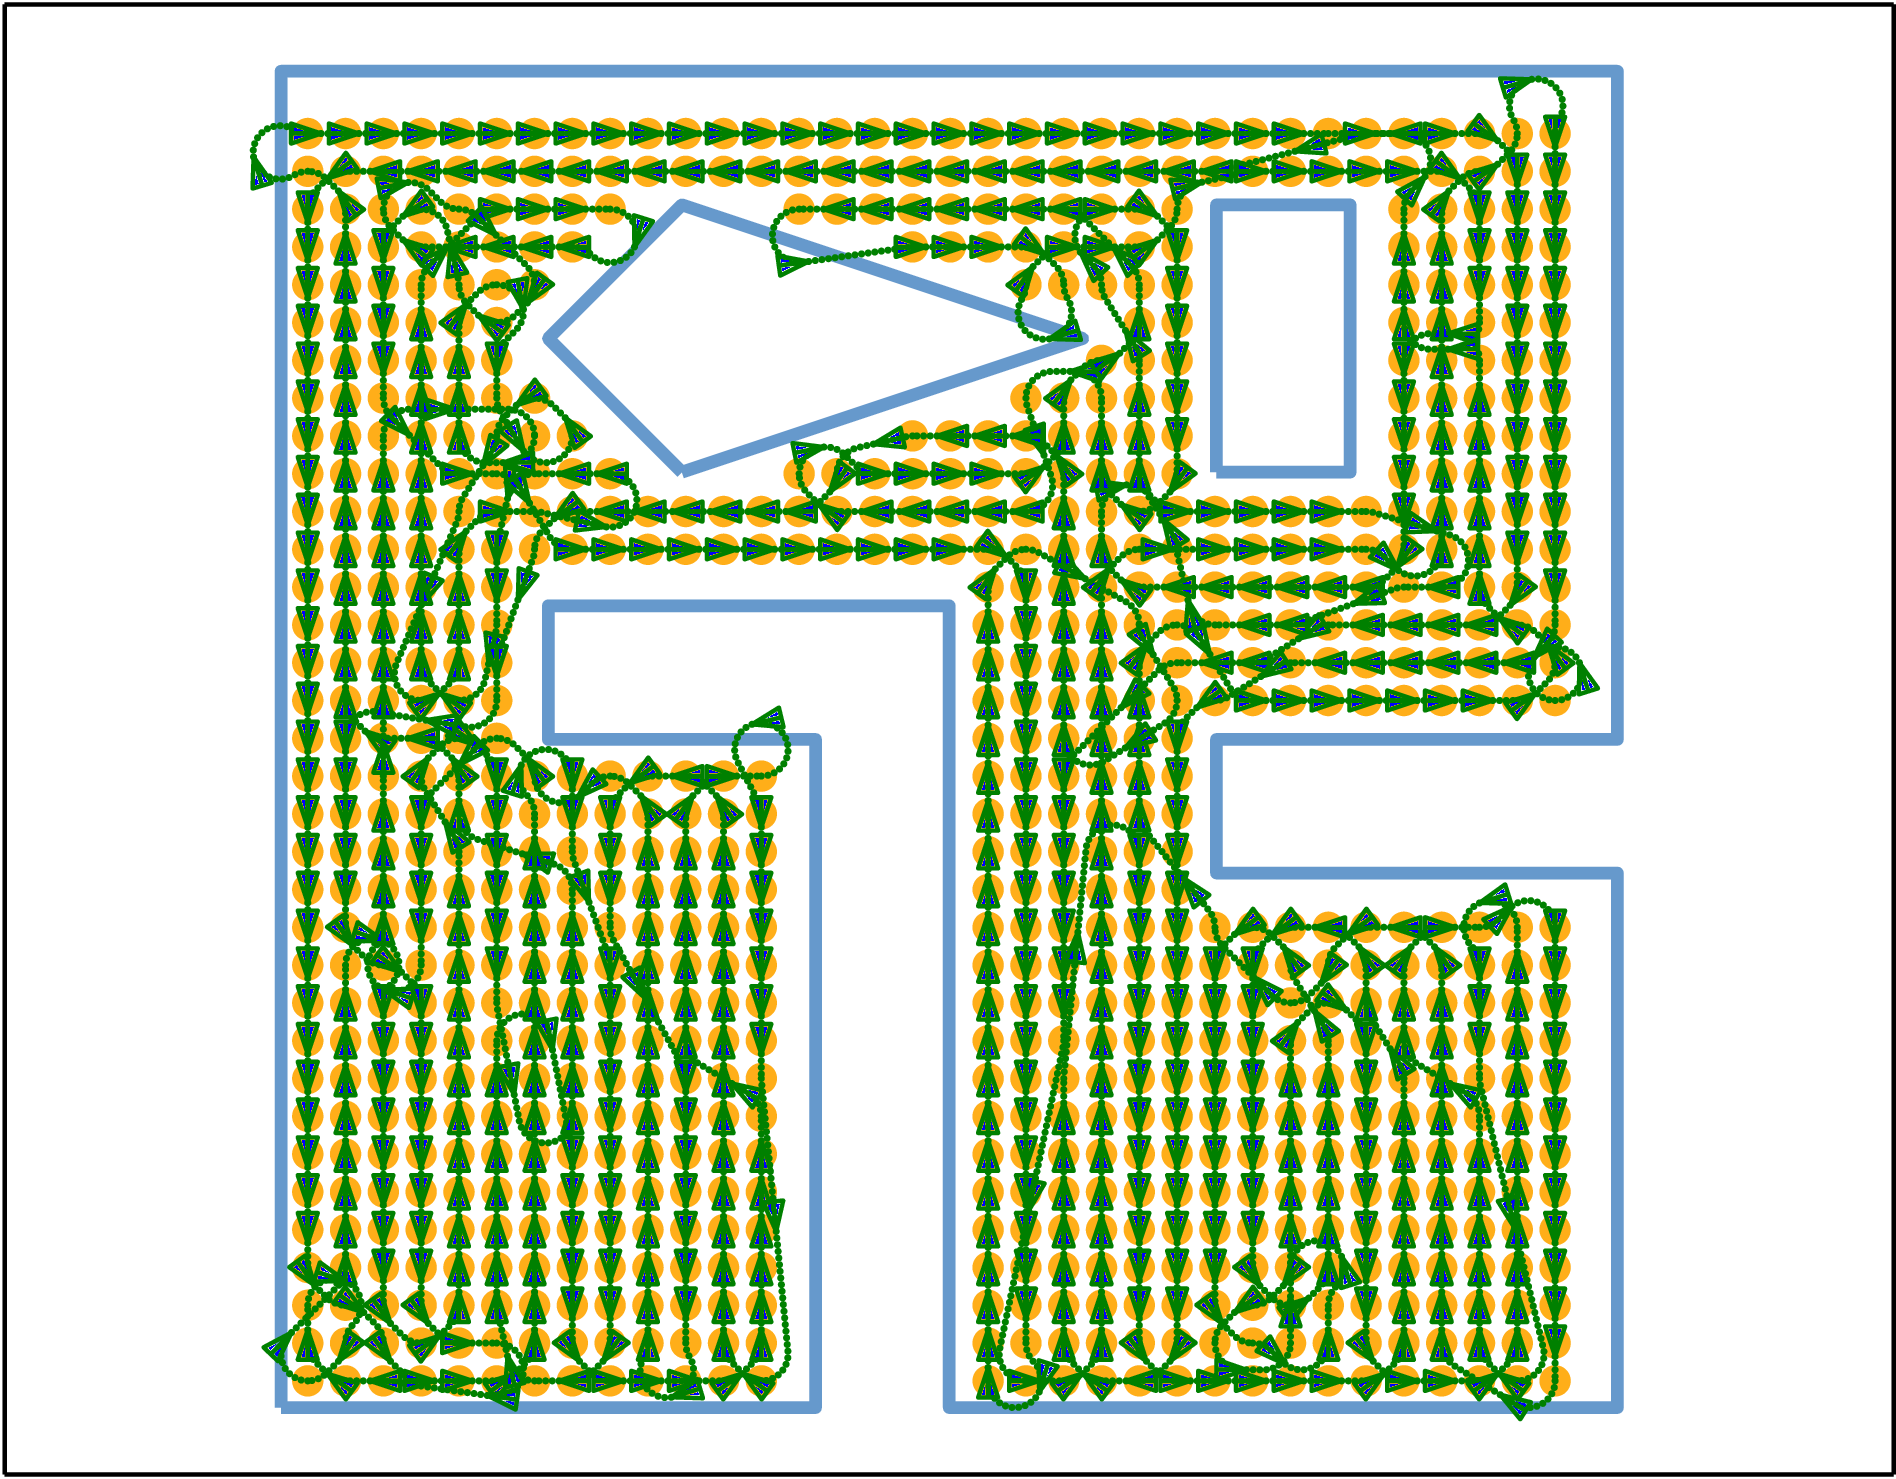
\includegraphics[width=0.3\textwidth]{img/chapter_3/point_13_coverage.png}%
		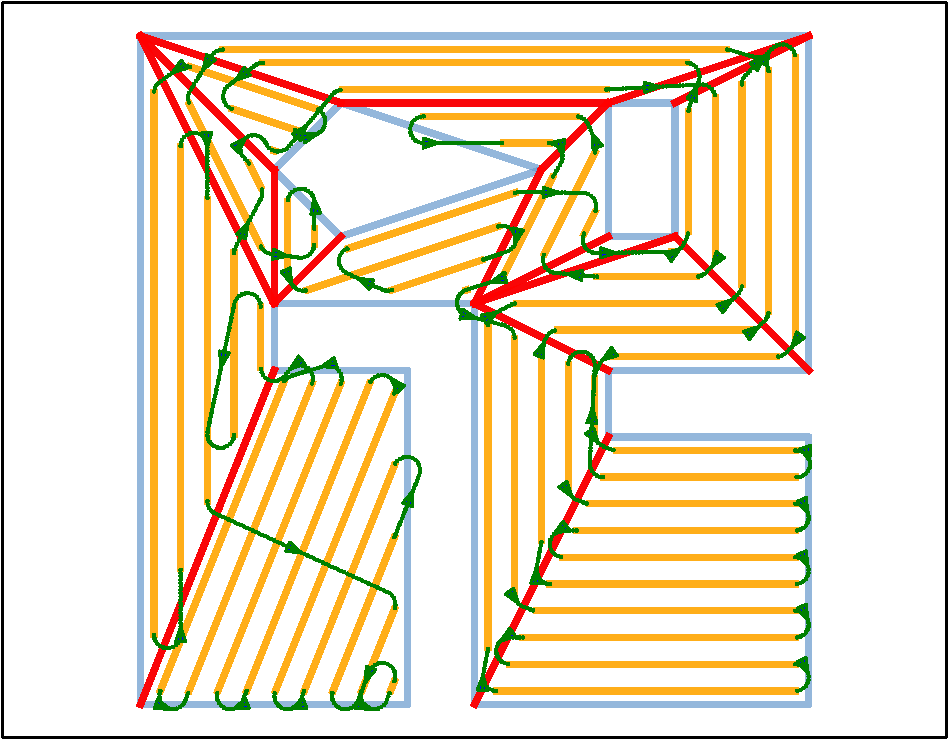
\includegraphics[width=0.3\textwidth]{img/chapter_3/greedy_13_coverage.pdf}% 
		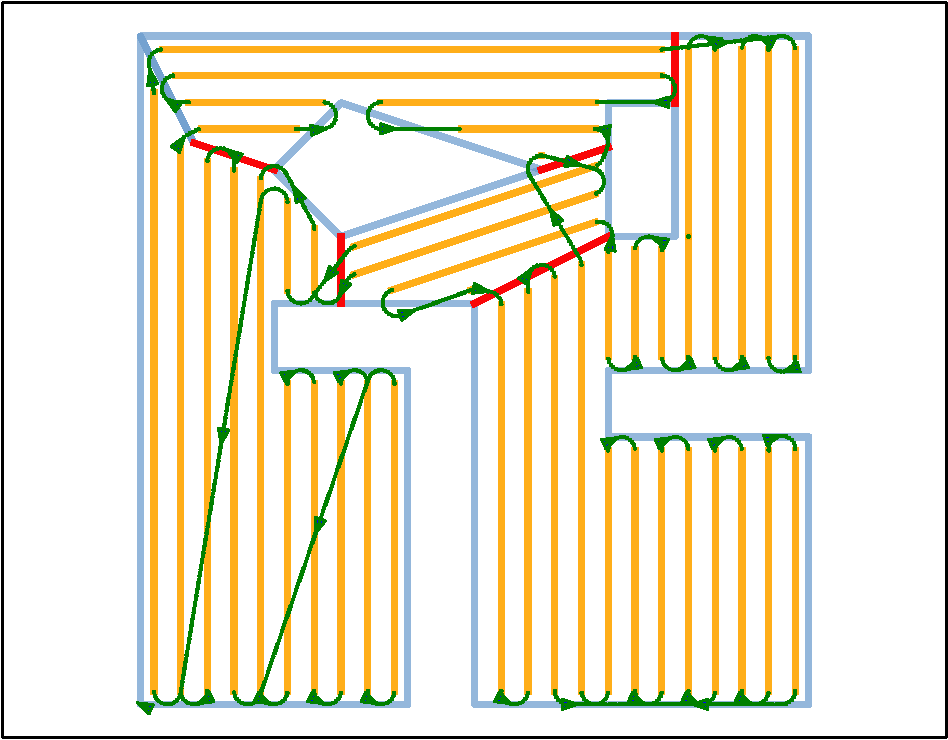
\includegraphics[width=0.3\textwidth]{img/chapter_3/min_13_coverage.pdf}
	\caption{First column: point decomposition. Second columm: greedy decomposition. Third column: min altitude decomposition.}
	\label{fig:coverage_results}
\end{figure*}

\end{document}